\documentclass{homework}

\usepackage[a4paper,margin=1in]{geometry}
\usepackage{kotex}
\usepackage{environ}
\usepackage{float}

\usepackage{amsmath}
\usepackage{amssymb}
\usepackage{braket}
\usepackage{intcalc}

\usepackage{graphicx}

\usepackage{tikz}
\usepackage[american]{circuitikz}
\usetikzlibrary{automata, positioning, arrows, shapes.gates.logic.US, shapes.gates.logic.IEC, calc}

\tikzset{
    node distance = 1.5cm,
    initial text = {},
    every state/.style = {
        thick,
        fill=gray!10
    },
    every edge/.style = {
        draw,
        ->, > = stealth',
        auto,
        semithick
    },
    dot/.style={
        minimum size = 3pt,
        inner sep = 0pt,
        fill,
        circle,
        node contents={}
    }
}

\usepackage{karnaugh-map}

\newcommand{\hwname}{이주헌}
\newcommand{\hwemail}{20191629}
\newcommand{\hwnum}{3}

\newcommand{\hwtype}{Homework}
\newcommand{\hwclass}{CSE3015}

\begin{document}

\maketitle

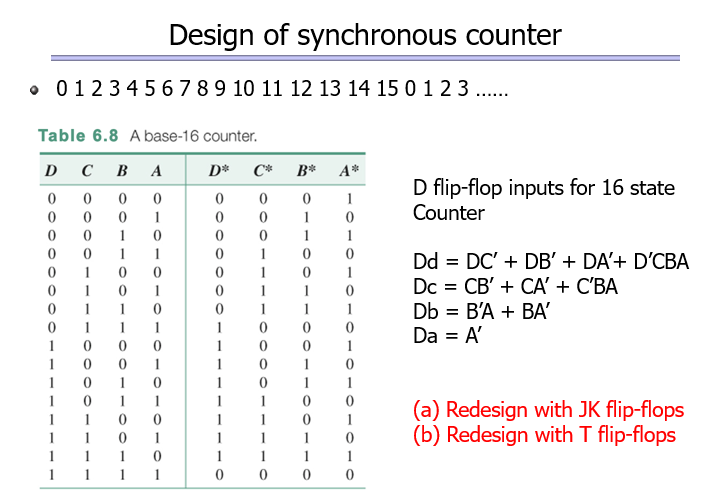
\includegraphics[width=\textwidth]{res/design-of-synchronous-counter.png}

\question*{Show each step how expressions for D flip-flop inputs are obtained.}

\begin{figure}[H]
\centering
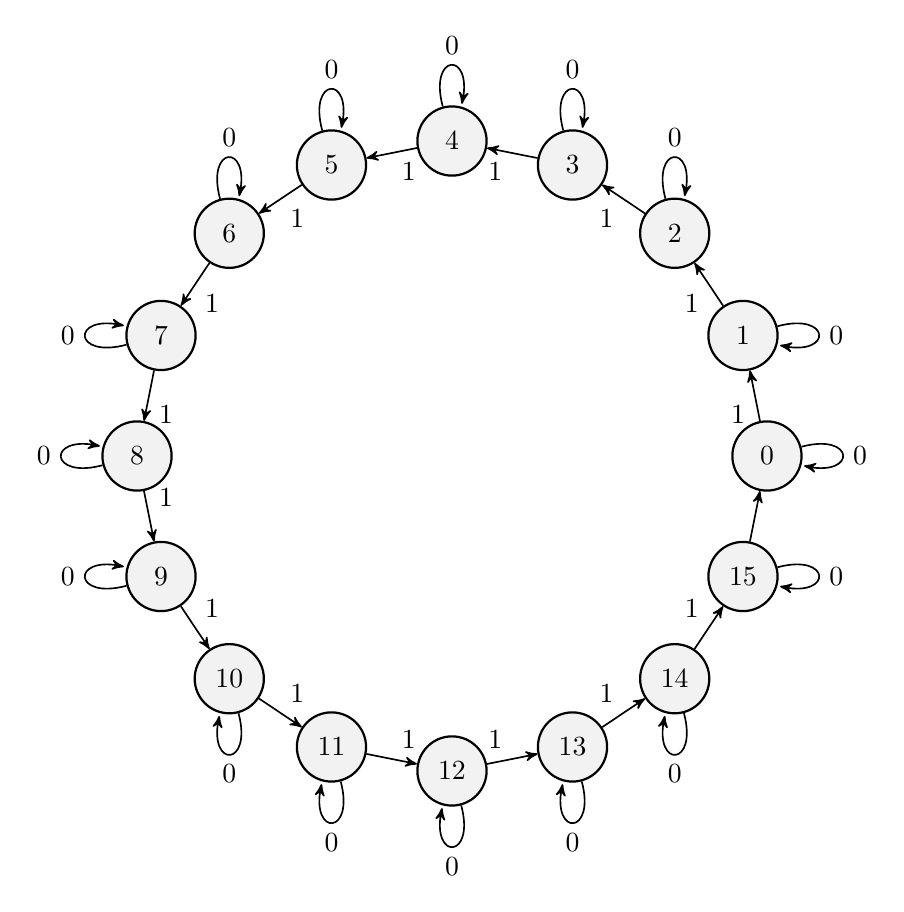
\begin{tikzpicture}
    \foreach \i in {0, 1, ..., 15}{
        \node[state] (\i) at ({\i * 360 / 16: 4cm}) {\i};
    }
    \foreach \i in {2, 3, ..., 6}{
        \draw (\i) edge[loop above] node{0} (\i);
    }
    \foreach \i in {7, 8, 9}{
        \draw (\i) edge[loop left] node{0} (\i);
    }
    \foreach \i in {10, 11, ..., 14}{
        \draw (\i) edge[loop below] node{0} (\i);
    }
    \foreach \i in {0, 1, 15}{
        \draw (\i) edge[loop right] node{0} (\i);
    }
    \foreach \i in {0, 1, ..., 14}{
        \draw (\i) edge node{1} (\the\numexpr\i+1\relax);
    }
    \draw (15) edge (0);
\end{tikzpicture}
\caption{State diagram of the 16-state counter.}
\label{fig:16-state-counter-diagram}
\end{figure}

\begin{table}[H]
\centering
\begin{tabular}{cccc|cccc|cccc}
D & C & B & A & D* & C* & B* & A* & $D_d$ & $D_c$ & $D_b$ & $D_a$ \\
\hline
0 & 0 & 0 & 0 & 0 & 0 & 0 & 1 & 0 & 0 & 0 & 1 \\
0 & 0 & 0 & 1 & 0 & 0 & 1 & 0 & 0 & 0 & 1 & 0 \\
0 & 0 & 1 & 0 & 0 & 0 & 1 & 1 & 0 & 0 & 1 & 1 \\
0 & 0 & 1 & 1 & 0 & 1 & 0 & 0 & 0 & 1 & 0 & 0 \\
0 & 1 & 0 & 0 & 0 & 1 & 0 & 1 & 0 & 1 & 0 & 1 \\
0 & 1 & 0 & 1 & 0 & 1 & 1 & 0 & 0 & 1 & 1 & 0 \\
0 & 1 & 1 & 0 & 0 & 1 & 1 & 1 & 0 & 1 & 1 & 1 \\
0 & 1 & 1 & 1 & 1 & 0 & 0 & 0 & 1 & 0 & 0 & 0 \\
1 & 0 & 0 & 0 & 1 & 0 & 0 & 1 & 1 & 0 & 0 & 1 \\
1 & 0 & 0 & 1 & 1 & 0 & 1 & 0 & 1 & 0 & 1 & 0 \\
1 & 0 & 1 & 0 & 1 & 0 & 1 & 1 & 1 & 0 & 1 & 1 \\
1 & 0 & 1 & 1 & 1 & 1 & 0 & 0 & 1 & 1 & 0 & 0 \\
1 & 1 & 0 & 0 & 1 & 1 & 0 & 1 & 1 & 1 & 0 & 1 \\
1 & 1 & 0 & 1 & 1 & 1 & 1 & 0 & 1 & 1 & 1 & 0 \\
1 & 1 & 1 & 0 & 1 & 1 & 1 & 1 & 1 & 1 & 1 & 1 \\
1 & 1 & 1 & 1 & 0 & 0 & 0 & 0 & 0 & 0 & 0 & 0
\end{tabular}
\caption{State table of the 16-state counter.}
\label{tab:16-state-counter-table}
\end{table}

\begin{table}[H]
\centering
\begin{tabular}{cc|c}
$Q_n$ & $Q_{n + 1}$ & $D$ \\
\hline
0 & 0 & 0 \\
0 & 1 & 1 \\
1 & 0 & 0 \\
1 & 1 & 1
\end{tabular}
\caption{Excitation table of the 16-state counter.}
\label{tab:16-state-counter-excitation-table}
\end{table}

\begin{figure}[H]
\centering
\begin{karnaugh-map}[4][4][1][$CD$][$AB$]
\minterms{2, 3, 6, 7, 10, 11, 13, 14}
\implicant{3}{6}
\implicantedge{3}{2}{11}{10}
\implicant{2}{10}
\implicant{13}{13}
\end{karnaugh-map}
\caption{$D_d = D \neg C + D \neg B + D \neg A + \neg DCBA$}
\label{fig:d-flip-flip-karnaugh-map-d}
\end{figure}

\begin{figure}[H]
\centering
\begin{karnaugh-map}[4][4][1][$CD$][$AB$]
\minterms{1, 3, 5, 7, 9, 11, 12, 14}
\implicant{1}{7}
\implicantedge{1}{3}{9}{11}
\implicantedge{12}{12}{14}{14}
\end{karnaugh-map}
\caption{$D_c = C \neg B + C \neg A + \neg CBA$}
\label{fig:d-flip-flip-karnaugh-map-c}
\end{figure}

\begin{figure}[H]
\centering
\begin{karnaugh-map}[4][4][1][$CD$][$AB$]
\minterms{4, 5, 6, 7, 8, 9, 10, 11}
\implicant{4}{6}
\implicant{8}{10}
\end{karnaugh-map}
\caption{$D_b = B \neg A + \neg BA$}
\label{fig:d-flip-flip-karnaugh-map-b}
\end{figure}

\begin{figure}[H]
\centering
\begin{karnaugh-map}[4][4][1][$CD$][$AB$]
\minterms{0, 1, 2, 3, 8, 9, 10, 11}
\implicantedge{0}{2}{8}{10}
\end{karnaugh-map}
\caption{$D_a = \neg A$}
\label{fig:d-flip-flip-karnaugh-map-a}
\end{figure}

% circuit diagram
\begin{figure}[H]
\begin{circuitikz}
    \ctikzset{multipoles/thickness=3}
    \ctikzset{multipoles/dipchip/width=2}
    
    \node (a) at (0, 0) {$A$};
    \node (b) at (1, 0) {$B$};
    \node (c) at (2, 0) {$C$};
    \node (d) at (3, 0) {$D$};
    \draw (a) -- ++(0, -4)
          (b) -- ++(0, -4)
          (c) -- ++(0, -4)
          (d) -- ++(0, -4);
    
    \node[dipchip, num pins=4, hide numbers, no topmark] (D1) at (4, -0.5) {D1};
\end{circuitikz}
\end{figure}

\question*{Redesign with JK flip-flops.}

\question*{Redesign with T flip-flops.}

\end{document}